% The four commands: three write declarations, one reads them. Built to fig_commands.pdf:
%   cd paper/figures && pdflatex fig_commands.tex
\documentclass[border=2pt]{standalone}
\usepackage[T1]{fontenc}
\usepackage{times}
\usepackage{tikz}
\usetikzlibrary{arrows.meta,positioning}

\definecolor{planline}{HTML}{9B59B6}
\definecolor{planfill}{HTML}{F5EEF8}
\definecolor{runline}{HTML}{3498DB}
\definecolor{runfill}{HTML}{EBF5FB}
\definecolor{citeline}{HTML}{E67E22}
\definecolor{citefill}{HTML}{FDF2E9}
\definecolor{checkline}{HTML}{27AE60}
\definecolor{checkfill}{HTML}{E9F7EF}
\definecolor{arrow}{HTML}{95A5A6}

\begin{document}
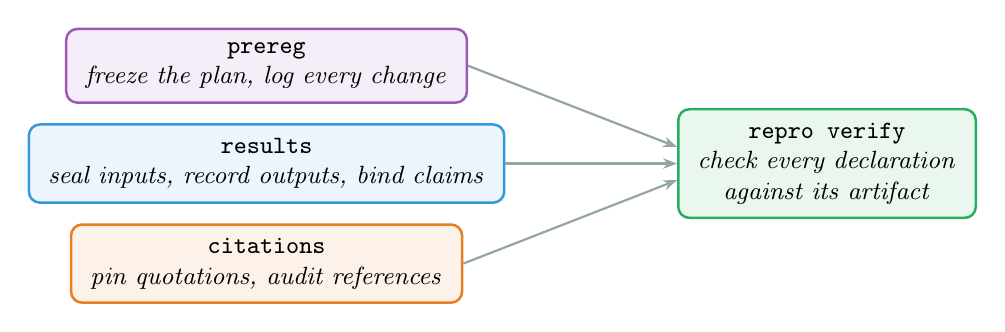
\begin{tikzpicture}[
  command/.style={draw=#1line, fill=#1fill, line width=0.9pt, rounded corners=4pt,
    align=center, inner xsep=7pt, inner ysep=5pt, font=\small},
  feeds/.style={-{Stealth[length=5pt]}, draw=arrow, line width=0.8pt},
]
  \node[command=run] (results) {\texttt{results}\\\textit{seal inputs, record outputs, bind claims}};
  \node[command=plan, above=7pt of results] (prereg) {\texttt{prereg}\\\textit{freeze the plan, log every change}};
  \node[command=cite, below=7pt of results] (citations) {\texttt{citations}\\\textit{pin quotations, audit references}};
  \node[command=check, right=62pt of results] (verify)
    {\texttt{repro verify}\\\textit{check every declaration}\\\textit{against its artifact}};
  \draw[feeds] (prereg.east) -- ([yshift=6pt]verify.west);
  \draw[feeds] (results.east) -- (verify.west);
  \draw[feeds] (citations.east) -- ([yshift=-6pt]verify.west);
\end{tikzpicture}
\end{document}
